\documentclass[spec, och, otchet, hidelinks]{SCWorks}
% параметр - тип обучения - одно из значений:
%    spec     - специальность
%    bachelor - бакалавриат (по умолчанию)
%    master   - магистратура
% параметр - форма обучения - одно из значений:
%    och   - очное (по умолчанию)
%    zaoch - заочное
% параметр - тип работы - одно из значений:
%    otchet
%    referat    - реферат
%    coursework - курсовая работа (по умолчанию)
%    diploma    - дипломная работа
%    pract      - отчет по практике
%    pract      - отчет о научно-исследовательской работе
%    autoref    - автореферат выпускной работы
%    assignment - задание на выпускную квалификационную работу
%    review     - отзыв руководителя
%    critique   - рецензия на выпускную работу
% параметр - включение шрифта
%    times    - включение шрифта Times New Roman (если установлен)
%               по умолчанию выключен
\usepackage[T2A]{fontenc}
\usepackage[utf8]{inputenc}
\usepackage{graphicx}

\usepackage[sort,compress]{cite}
\usepackage{amsmath}
\usepackage{amssymb}
\usepackage{amsthm}
\usepackage{fancyvrb}
\usepackage{longtable}
\usepackage{array}
\usepackage[english,russian]{babel}
\usepackage{minted}
% Используется автором репозитория
%\usemintedstyle{xcode}
% Этот пакет включает в себя аналогичный Times New Roman шрифт.
% Необходим для успешной компиляции для UNIX-систем ввиду отсутствия TNR в нем.
% Можно использовать и для Windows.
\usepackage{tempora}


\usepackage[colorlinks=false]{hyperref}

\graphicspath{{figures/}}

\newcommand{\eqdef}{\stackrel {\rm def}{=}}

\usepackage{stackengine}
\newcommand\xrowht[2][0]{\addstackgap[.5\dimexpr#2\relax]{\vphantom{#1}}}

\newtheorem{lem}{Лемма}

% % При использовании biblatex вместо bibtex
%\usepackage[style=gost-numeric]{biblatex}
%\addbibresource{thesis.bib}

\begin{document}

% Кафедра (в родительном падеже)
\chair{математической кибернетики и компьютерных наук}

% Тема работы
\title{Счётчики}

% Курс
\course{3}

% Группа
\group{331}

% Факультет (в родительном падеже) (по умолчанию "факультета КНиИТ")
%\department{факультета КНиИТ}

% Специальность/направление код - наименование
%\napravlenie{02.03.02 "--- Фундаментальная информатика и информационные технологии}
%\napravlenie{02.03.01 "--- Математическое обеспечение и администрирование информационных систем}
%\napravlenie{09.03.01 "--- Информатика и вычислительная техника}
%\napravlenie{09.03.04 "--- Программная инженерия}
\napravlenie{10.05.01 "--- Компьютерная безопасность}

% Для студентки. Для работы студента следующая команда не нужна.
%\studenttitle{Студентки}

% Фамилия, имя, отчество в родительном падеже
\author{Бородина Артёма Горовича}

% Заведующий кафедрой
\chtitle{доцент, к.\,ф.-м.\,н.} % степень, звание
\chname{С.\,В.\,Миронов}

%Научный руководитель (для реферата преподаватель проверяющий работу)
\satitle{аспирант}%, к.\,ф.-м.\,н.} %должность, степень, звание
\saname{А.\,А.\,Мартышкин}

% Руководитель практики от организации (только для практики,
% для остальных типов работ не используется)
\patitle{к.\,ф.-м.\,н., доцент}
\paname{Д.\,Ю.\,Петров}

% Семестр (только для практики, для остальных
% типов работ не используется)
\term{2}

% Наименование практики (только для практики, для остальных
% типов работ не используется)
\practtype{учебная}

% Продолжительность практики (количество недель) (только для практики,
% для остальных типов работ не используется)
\duration{2}

% Даты начала и окончания практики (только для практики, для остальных
% типов работ не используется)
\practStart{01.07.2016}
\practFinish{14.07.2016}

% Год выполнения отчета
\date{2022}

\maketitle

% Включение нумерации рисунков, формул и таблиц по разделам
% (по умолчанию - нумерация сквозная)
% (допускается оба вида нумерации)
%\secNumbering


\tableofcontents

% Раздел "Обозначения и сокращения". Может отсутствовать в работе
% \abbreviations
% \begin{description}
%     \item ... "--- ...
%     \item ... "--- ...
% \end{description}

% Раздел "Определения". Может отсутствовать в работе
%\definitions

% Раздел "Определения, обозначения и сокращения". Может отсутствовать в работе.
% Если присутствует, то заменяет собой разделы "Обозначения и сокращения" и "Определения"
%\defabbr


% Раздел "Введение"

\intro

Целью данной работы служит ознакомление с устройством и функционированием счетчиков, а также испытание синхронного суммирующего, реверсивного и 
десятичного счетчиков.

\newpage

\section*{Задание 1.}
\addcontentsline{toc}{section}{Задание 1}

Запустить лабораторный комплекс Labworks и среду МS10. Открыть файл \textbf{34.6.ms10}, размещенный в папке \textbf{Circuit Design Suitе 10.0} среды 
МS10, или собрать на рабочем поле среды MS10 схему для испытания \textit{синхронного двоичного счетчика} и установить в диалоговых окнах компонентов 
их параметры или режимы работы. \textbf{Скопировать} схему в отчет.

\begin{figure}[h]
	\center{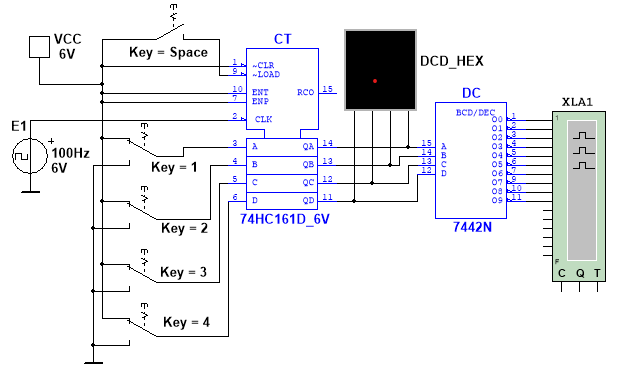
\includegraphics{scheme_task_one.png}}
	\caption{Схема синхронного двоичного счётчика.}
\end{figure}

\newpage

\section*{Задание 2.}
\addcontentsline{toc}{section}{Задание 2}

\textbf{Замкнуть} ключ \textbf{Space}, \textbf{запустить} программу моделирования суммирующего счетчика и \textbf{наблюдать} за показаниями индикатора.
\textbf{Убедиться}, что на экране анализатора \textbf{XLA1} логические нули перестают формироваться после прихода 11-го тактового импульса и появляются 
вновь только с приходом 17-го импульса.

\begin{figure}[h]
	\center{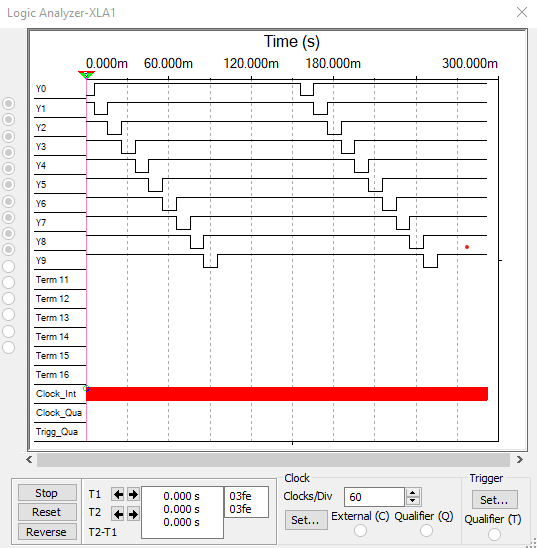
\includegraphics{logic_analyzer_task_two_zeros.png}}
	\caption{Показания индикатора при замкнутом ключе \textbf{Space}.}
\end{figure}

\newpage

\textbf{Разомкнуть} ключ \textbf{Space}. \textbf{Установить} в диалоговом окне анализатора \textbf{XLA}1 напряжение \textbf{V} = 5 B, частоту таймера 
$ f_\text{a} $ = 2 кГц, число импульсов, приходящихся на одно деление, \textbf{Clocks/div} = 60. С помощью активных клавиш 1, 2, 3 и 4 клавиатуры 
\textbf{сформировать} произвольные двоичные входные числа (коды) и \textbf{подавать} их на входы \textbf{D, С, В и А} счетчика. \textbf{Убедиться}, 
что при подаче числа $ 1110_2 $ ни на одном выходе дешифратора 4х10 не сформировался низкий уровень сигнала. 

\par Подадим на входы двоичные числа, соответствующие 4, 8 и 14 в десятичной системе:

\begin{figure}[h]
	\center{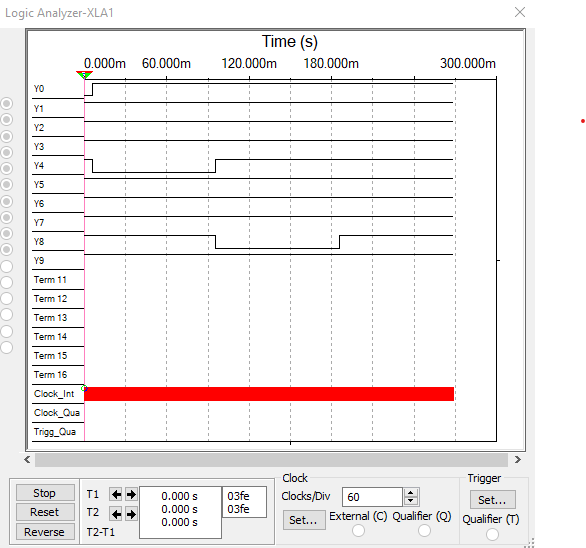
\includegraphics{arbitrary_binary_sequences.png}}
	\caption{Подача на вход счётчика произвольных двоичных чисел.}
\end{figure}

Действительно, при обработке числа $ 14_{10} $ ни на одном из выходов дешифратора не сформировалось низкого уровня сигнала. 

\newpage

\section*{Задание 3.}
\addcontentsline{toc}{section}{Задание 3}

Открыть файл \textbf{34.8.ms10}, размещенный в папке \textbf{Circuit Design Suitе 10.0} среды МS10, или собрать на рабочем поле среды MS10 схему для 
испытания \textit{реверсивного двоичного счетчика} и установить в диалоговых окнах компонентов их параметры или режимы работы. \textbf{Скопировать} схему в отчет.

\begin{figure}[h]
	\center{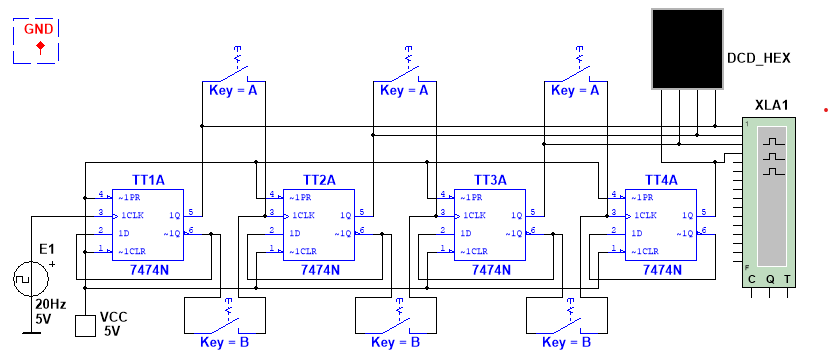
\includegraphics[scale=0.8]{scheme_task_three.png}}
	\caption{Схема реверсивного двоичного счётчика.}
\end{figure}

\textbf{Установить} в диалоговом окне анализатора \textbf{XLA1} напряжение \textbf{V} = 5 B, частоту таймера $ f_\text{a} $ = 2 кГц, число импульсов, 
приходящихся на одно деление, \textbf{Clocks/div} = 60. \textbf{Разомкнуть} ключи \textbf{В} и \textbf{замкнуть} ключи А. \textbf{Запустить} программу 
моделирования счетчика. При высвечивании числа 15 на 7-сегментном индикаторе \textbf{щелкнуть мышью} на кнопке \textbf{Stop} (остановки моделирования) и 
\textbf{скопировать} окно анализатора с результатами моделирования в отчет.

\newpage

\begin{figure}[h]
	\center{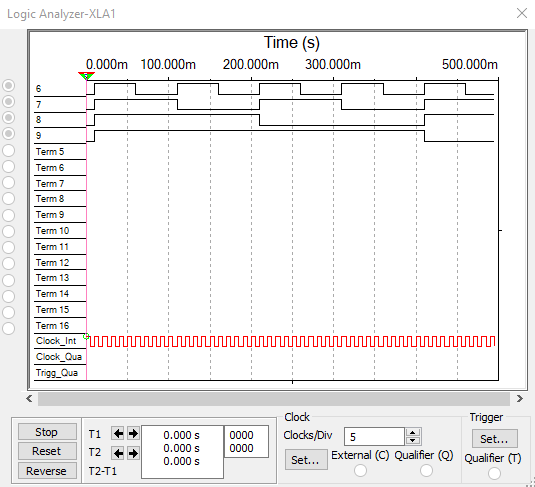
\includegraphics[scale=0.8]{counter_program_model_task_three_first.png}}
	\caption{Результаты моделирования на первой части последовательности.}
\end{figure}

\begin{figure}[h!]
	\center{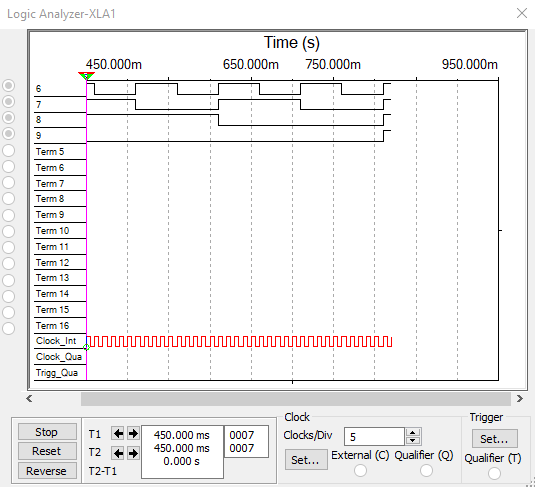
\includegraphics[scale=0.8]{counter_program_model_task_three_second.png}}
	\caption{Результаты моделирования на второй части последовательности.}
\end{figure}

\newpage

\textbf{Разомкнуть} ключи \textbf{А} и \textbf{замкнуть} ключи \textbf{В}. \textbf{Щелкнуть мышью} на кнопке \textbf{Stop}, \textbf{остановить} 
моделирование при высвечивании числа 0 на индикаторе и \textbf{скопировать} окно анализатора с результатами моделирования в отчет.

\begin{figure}[h]
	\center{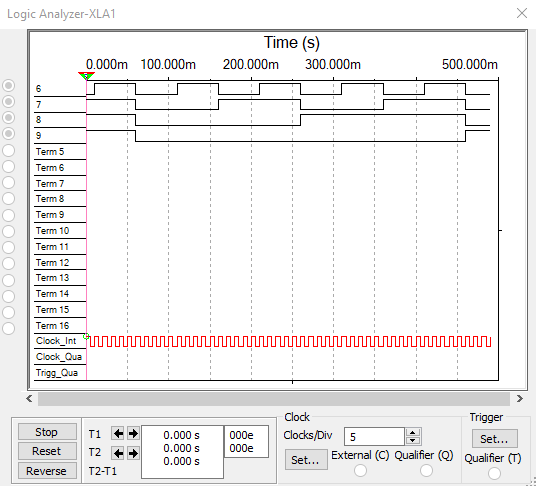
\includegraphics[scale=0.78]{counter_program_model_task_three_first_reverse.png}}
	\caption{Результаты моделирования на первой части последовательности.}
\end{figure}

\begin{figure}[h!]
	\center{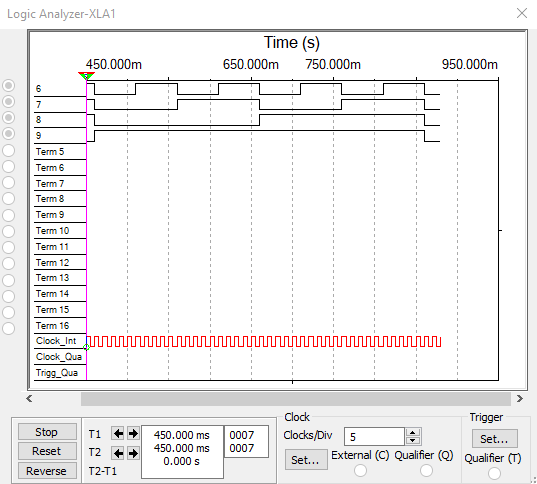
\includegraphics[scale=0.78]{counter_program_model_task_three_second_reverse.png}}
	\caption{Результаты моделирования на второй части последовательности.}
\end{figure}

\newpage

\section*{Задание 4.}
\addcontentsline{toc}{section}{Задание 4}

Открыть файл \textbf{34.10.ms10}, размещенный в папке \textbf{Circuit Design Suitе 10.0} среды МS10, или собрать на рабочем поле среды MS10 схему для 
испытания \textit{десятичного счетчика} и установить в диалоговых окнах компонентов их параметры или режимы работы. \textbf{Скопировать} схему в отчет.

\begin{figure}[h]
	\center{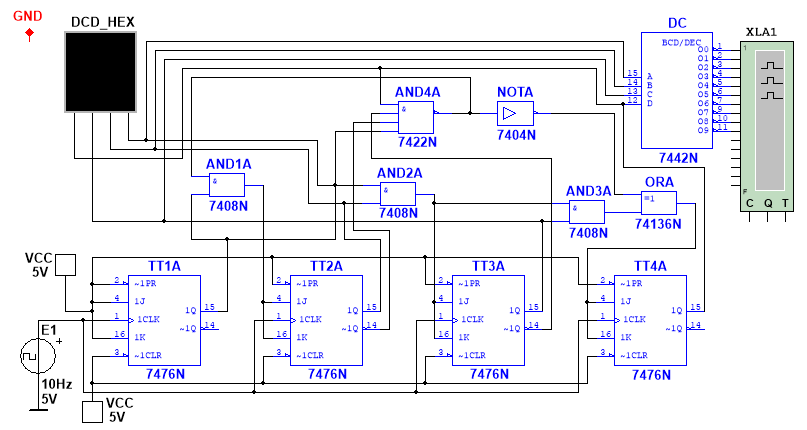
\includegraphics[scale=0.8]{scheme_task_four.png}}
	\caption{Схема десятичного счётчика.}
\end{figure}

\newpage

\textbf{Запустить} программу моделирования десятичного счетчика и \textbf{скопировать} окно анализатора с результатами моделирования в отчет.

\begin{figure}[h]
	\center{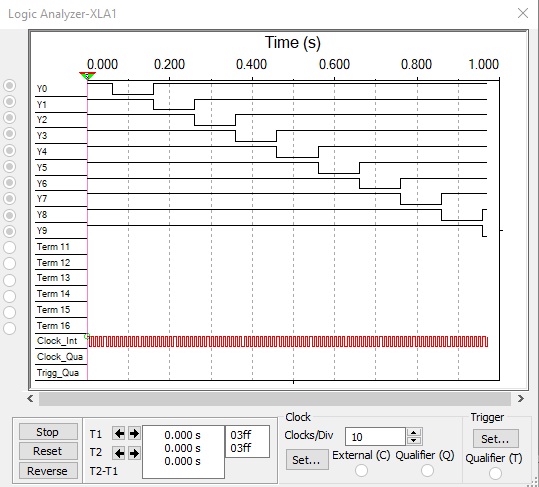
\includegraphics{window_task_four_first.png}}
	\caption{Результат программы моделирования десятичного счётчика.}
\end{figure}

\newpage

\section*{Тестовые задания.}
\addcontentsline{toc}{section}{Тестовые задания}

\par 1. Укажите, в \textbf{каком виде} фиксируется в счетчике число поступивших на его вход импульсов: \textbf{в виде двоичного кода, хранящегося в 
триггерах};

\par 2. Укажите необходимое \textbf{число выходов} двоичного счетчика для выдачи результатов
счета 28 импульсов: \textbf{4};

\par 3. Укажите, в \textbf{какой момент} 5-разрядный двоичный счетчик возвращается в начальное состояние: \textbf{при подаче на вход 32-го импульса};

\par 4. На 7-сегментном индикаторе десятичного счетчика высвечивается число 5. Укажите, какое \textbf{число} будет высвечиваться на индикаторе при 
подаче на вход еще шести импульсов: \textbf{3};

\par 5. Укажите, \textbf{каким путем передаются сигналы} от разряда к разряду в синхронном
счетчике: \textbf{посредством специальной переключающей схемы};

\par 6. Укажите, что понимают под \textbf{коэффициентом пересчета} счетчика: \textbf{это модуль счета, характеризуемый числом устойчивых состояний счетчика};

\par 7. Укажите, чему равен \textbf{модуль M пересчета} двоичного п-разрядного счетчика: \textbf{$ M = 2 ^ n $};

\par 8. Укажите, сколько \textbf{триггеров} должен иметь двоично-кодированный счетчик с коэффициентом пересчета $ M = 8 $: \textbf{3};

\par 9. Укажите \textbf{пути и средства}, с помощью которых изменяется направление счета в реверсивном счетчике: \textbf{направление счёта изменяется путём изменения вида межразрядных связей}.

\newpage

\conclusion

В ходе данной лабораторной работы мы ознакомились с устройством и функционированием счётчиков, а также испытали синхронный, суммирующий, реверсивный 
и десятичный счётчики на практике.

\end{document}